\documentclass{article}


\usepackage{arxiv}

\usepackage[utf8]{inputenc} % allow utf-8 input
\usepackage[T1]{fontenc}    % use 8-bit T1 fonts
\usepackage{hyperref}       % hyperlinks
\usepackage{url}            % simple URL typesetting
\usepackage{booktabs}       % professional-quality tables
\usepackage{amsfonts}       % blackboard math symbols
\usepackage{nicefrac}       % compact symbols for 1/2, etc.
\usepackage{microtype}      % microtypography
\usepackage{amsmath}
\usepackage{array}
\usepackage{amssymb}
\usepackage{bm}
\usepackage{graphicx}
\usepackage{rotating}
\graphicspath{ {./} }

\title{Tutorial on Neural Network Math for Forward Propagation and Backward Propagation}

\author{
  Kyle Bradbury \\
  Energy Initiative\\
  Duke University\\
  \texttt{kyle.bradbury@duke.edu} \\
%   %% examples of more authors
%   \And
%  Elias D.~Striatum \\
%   Department of Electrical Engineering\\
%   Mount-Sheikh University\\
%   Santa Narimana, Levand \\
%   \texttt{stariate@ee.mount-sheikh.edu} \\
% David S.~Hippocampus\thanks{Use footnote for providing further
%     information about author (webpage, alternative
%     address)---\emph{not} for acknowledging funding agencies.} \\
}

\begin{document}
\maketitle

\begin{abstract}
There is no better way of understanding the how neural networks are applied and trained than by coding up a simple version of one. Here we walk through a simple neural network providing equations (and matrix expressions) for calculating each component of a feedforward neural network and all of the necessary equations to implement in code both forward and backward propagation to apply and train a neural network.
\end{abstract}


% keywords can be removed
\keywords{Machine learning \and matrix algebra \and backpropagation \and neural networks \and quick reference}

\section{Introduction}

In supervised machine learning our goal is find a function that best maps our input, $\mathbf{x}_n$ to our output(s) $\mathbf{y}_n$. We typically do this by finding the function that best accomplishes this mapping: $\mathbf{y}_n = f(\mathbf{x}_n, \mathbf{w})$, where $\mathbf{w}$ are the parameters of our model, $f$. To find the function that does this best, we adjust we adjust the model parameters to minimize our error. Neural networks are one choice of function for accomplishing supervised learning and we also simply pick the weight parameters, $\mathbf{w}$, for our network that minimize the error.

To do this, we typically need to find the gradient (derivative) of the error function with respect to each parameter in the model (the weights) and when possible, set the gradient equal to zero, but in the case of neural networks, since there's no closed-form solution, we move in the direction of steepest descent (the opposite direction of the gradient). But how do we calculate the gradient of these networks? To do so, we use backpropagation, which essentially accounts for impact that each of the weights has one the error of the neural network. Backpropagation is simply the process of using the chain rule of differentiation to walk backwards through a neural network and calculate the partial derivative of the error with respect to each parameter.

In this tutorial, we walk through the intuition behind backpropagation, some basic examples, and then a small neural network and walk through each step in the process. That will build up to a presentation of the more general equations for backpropagation that can be applied to any size neural network as well as some matrix representations of those equations to make the implementation easier. The goal is for you to have the tools you need to implement your own simple neural network by the end of this tutorial.

\section{The joy of the chain rule}

Let's say $z=f(y)$ and $y=g(x)$ and we want to know the derivative of $z$ with respect to $x$. By the chain rule we know how to calculate this:

\begin{equation}
    \dfrac{\partial z}{\partial x} = \dfrac{\partial z}{\partial y} \dfrac{\partial y}{\partial x}
\end{equation}

\begin{figure}[h]
\centering
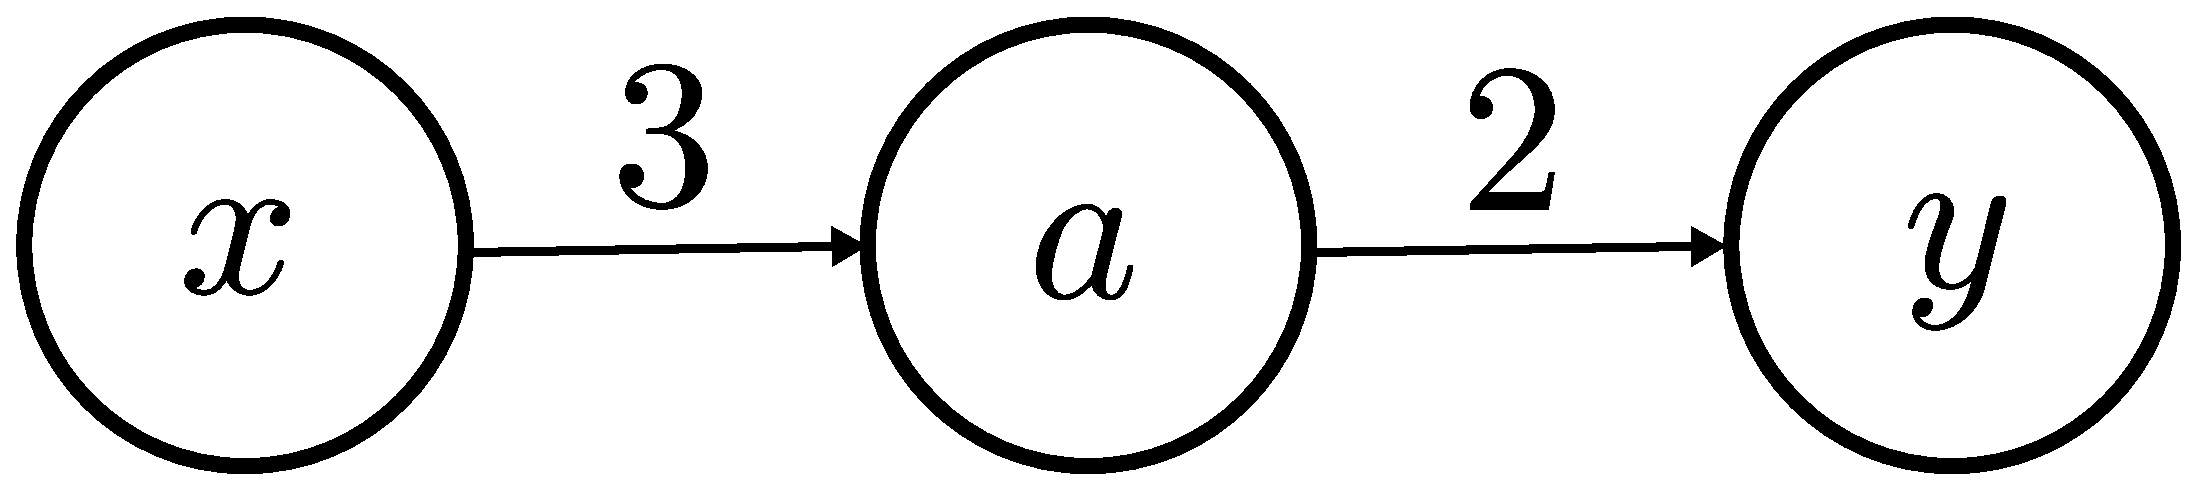
\includegraphics[width=0.3\textwidth]{./neural_networks_gradients_ex1.eps}
\caption{Example neural network}
\label{fig:ex1}
\end{figure}

Consider the simple case in Figure \ref{fig:ex1}. Here we use a graphical representation where each node (or vertex) is a value and the paths between nodes (or edges) is represented by a constant multiplied by the value from the previous node. So we can write these equations as:
\begin{align}
    y &= 2a \\
    a &= 3x
\end{align}

Of course, we could compose these functions and simply write $y=6x$, but we'll show the chain rule in this simplest case and quickly add complexity. We can write out the local derivatives for nodes $a$ and $y$.

\begin{align}
    \dfrac{\partial y}{\partial a} &= 2 \\
    \dfrac{\partial a}{\partial x} &= 3
\end{align}

Using the chain rule we have that

\begin{equation}
    \dfrac{\partial y}{\partial x} = \dfrac{\partial y}{\partial a} \dfrac{\partial a}{\partial x} = (2)(3) = 6
\end{equation}

As we move backward along a path, we apply the chain rule to "propagate" the derivative (the gradient) backwards through the graph. This is a key takeaway: along a path, we apply the chain rule.

\begin{figure}[h]
\centering
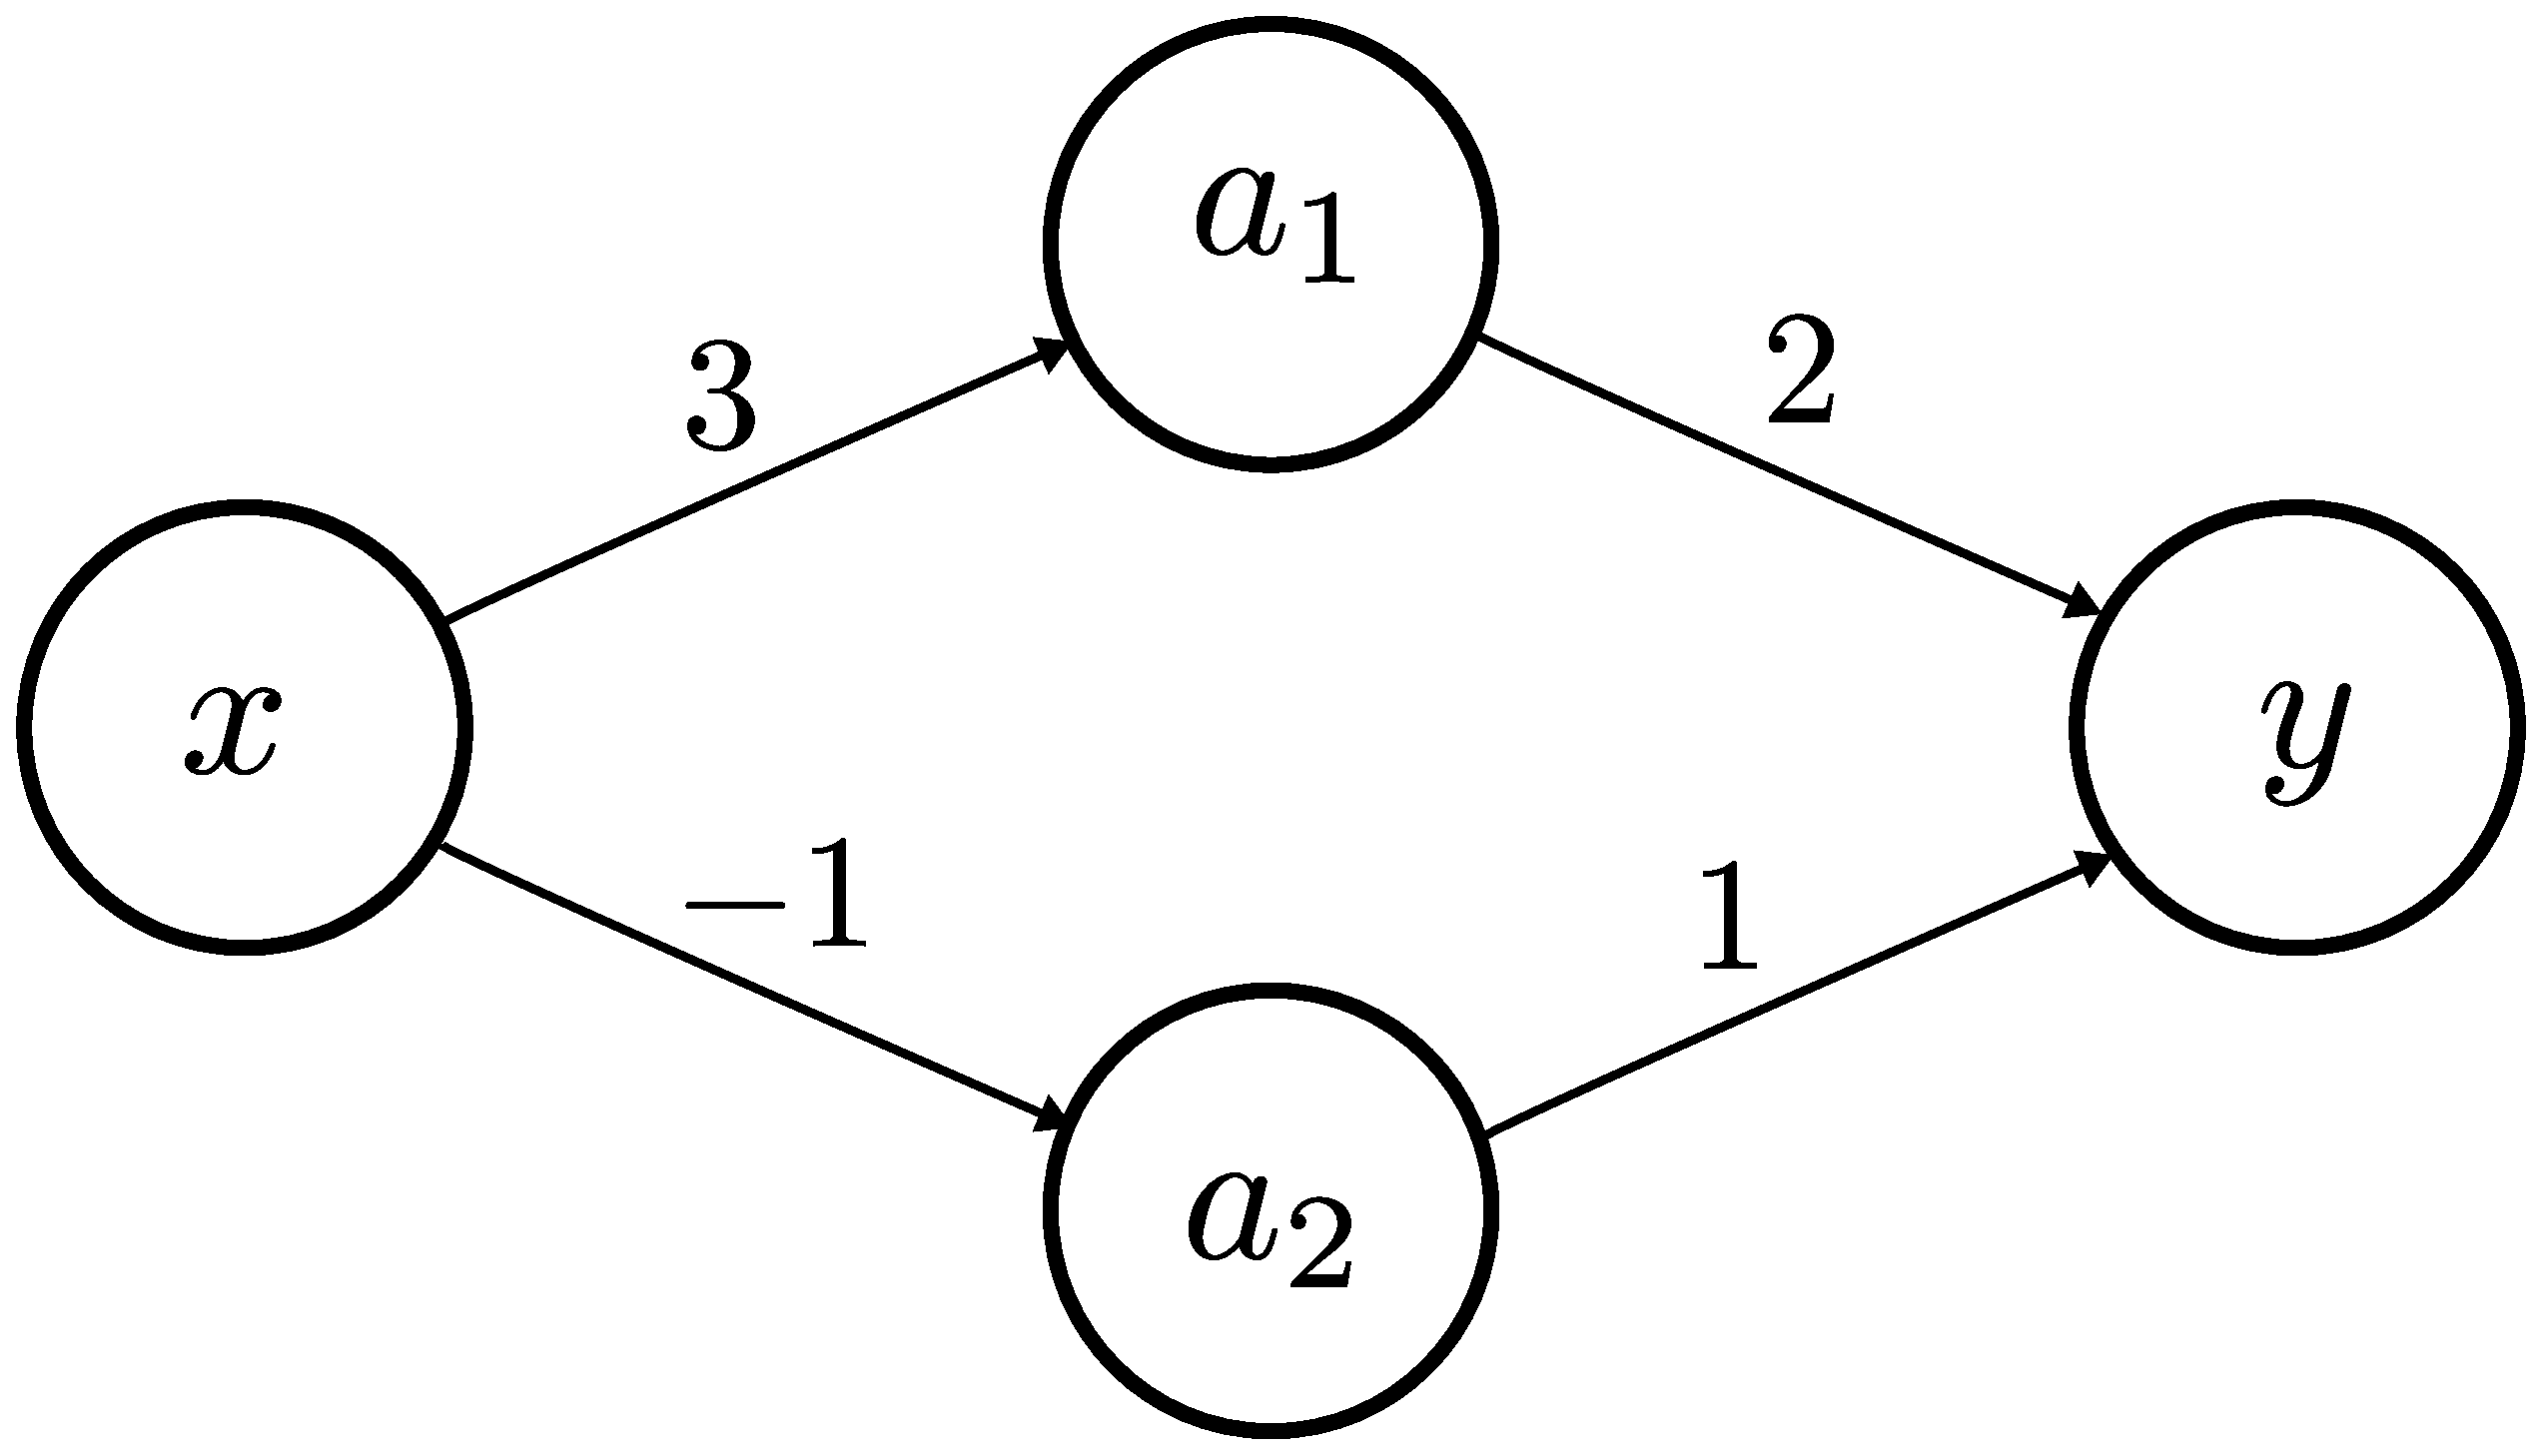
\includegraphics[width=0.3\textwidth]{./neural_networks_gradients_ex2.eps}
\caption{Example neural network}
\label{fig:ex2}
\end{figure}

In neural networks, we don't typically have this straight line from left to right, instead, there are multiple parallel pathways. Consider the example in \ref{fig:ex2}. Here we can write out our three local equations for nodes $y$, $a_1$, and $a_2$:

\begin{align}
    y &= 2a_1 + a_2 \\
    a_1 &= 3x \\
    a_2 &= -x
\end{align}

If we tried to apply the chain rule directly, the fact that there are multiple paths connecting $x$ to $y$ becomes a challenge. But here we can use another important rule in calculus, the sum rule for differentiation:

\begin{equation}
    \dfrac{\partial}{\partial x} (a_1 + a_2) = \dfrac{\partial a_1}{\partial x} + \dfrac{\partial a_2}{\partial x}
\end{equation}

We can then apply the chain rule to $\frac{\partial a_1}{\partial x}$ and $\frac{\partial a_2}{\partial x}$ to get the derivative with respect to $x$:

\begin{equation}
\begin{split}
    \frac{\partial y}{\partial x} &= \frac{\partial y}{\partial a_1} \frac{\partial a_1}{\partial x} + \frac{\partial y}{\partial a_2} \frac{\partial a_2}{\partial x} \\
    &= (2)(3) + (1)(-1) \\
    &= 5
\end{split}
\end{equation}

To make sure this makes sense, we see that if we substitute in the values for $a_1$ and $a_2$ we get that $y=2(3x) - x = 5x$. Here we can clearly see that the derivative of $y$ with respect to $x$ is 5.

A key takeaway here is that when we encounter multiple parallel paths from one node to another, as in \ref{fig:ex2}, we have to add the contribution of the derivative from each of the paths that come out of one node. This combination of the sum rule and the chain rule for differentiation allow us to calculate the gradients in many different graphs where nodes feed forward into one another sequentially, such as with feedforward neural networks.

\begin{figure}[h]
\centering
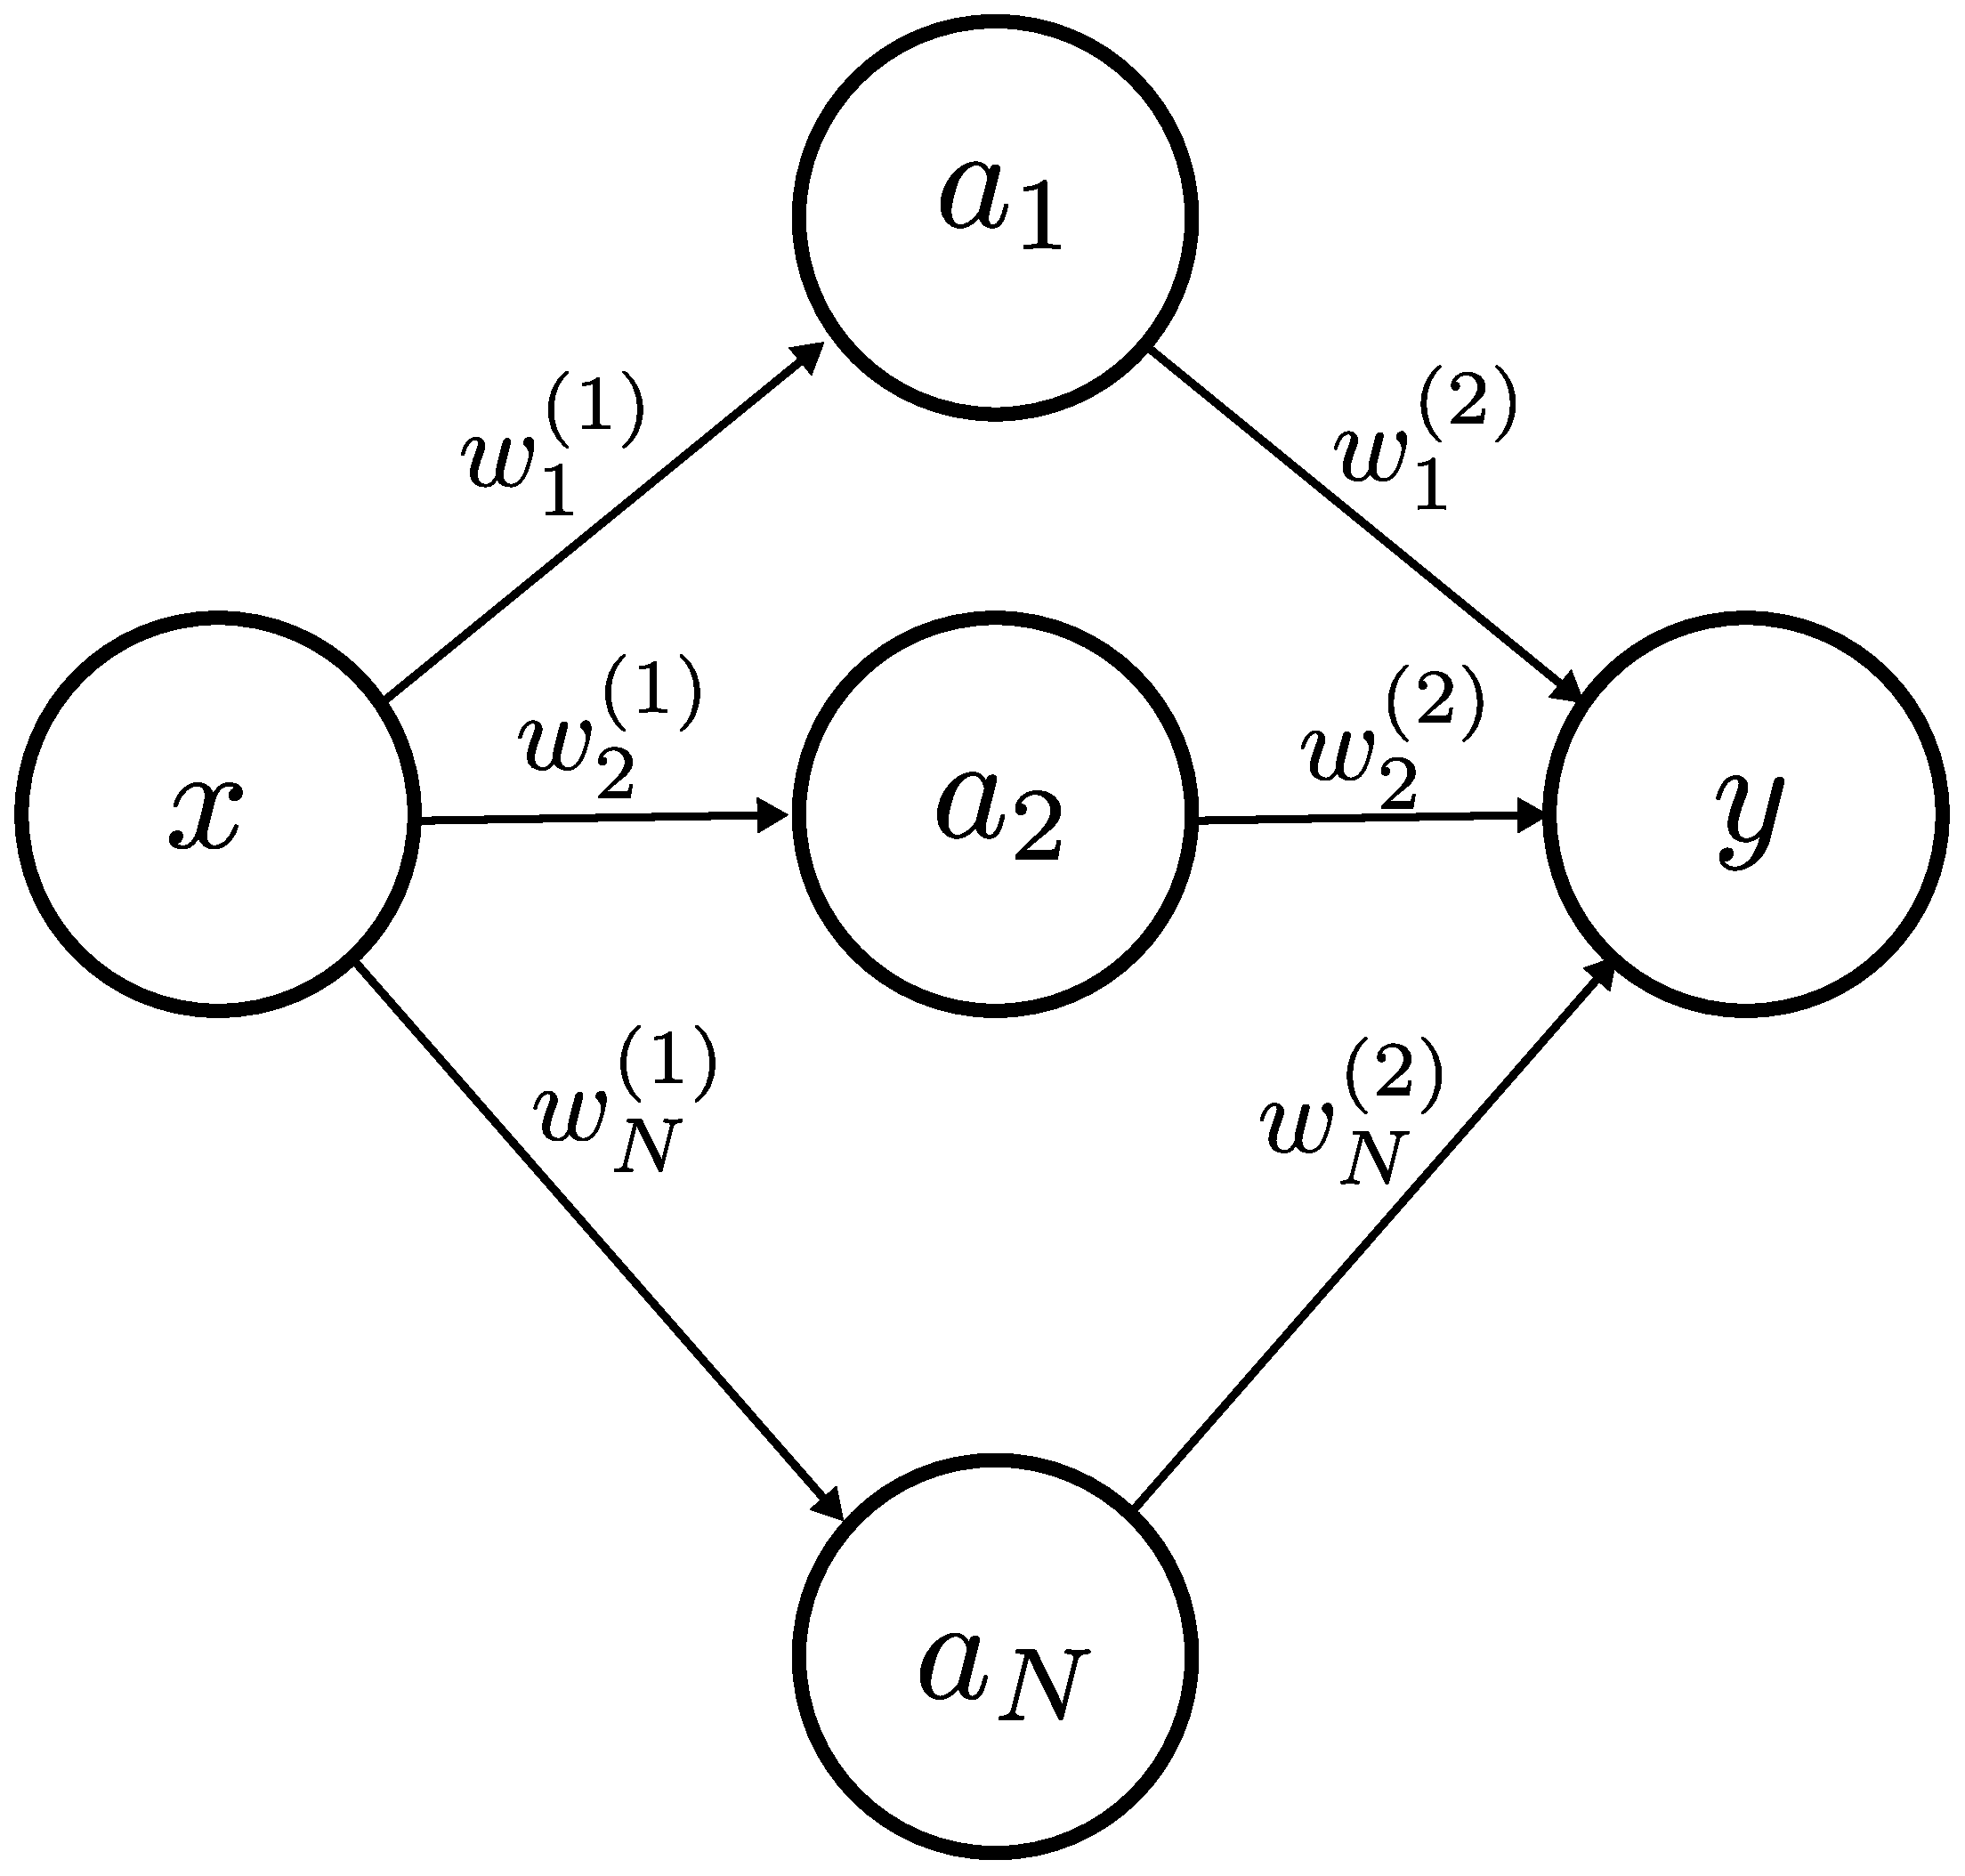
\includegraphics[width=0.3\textwidth]{./neural_networks_gradients_ex3.eps}
\caption{Example neural network}
\label{fig:ex3}
\end{figure}

Let's go through one slightly more complex example to get us ready for applying this directly to neural networks. Consider the situation in \ref{fig:ex3} that has $N$ paths from $x$ to $y$ instead of the earlier situations with only one or two described previously. Here the same combination of the sum rule across paths and the chain rule along paths can be applied. Let's start by righting our the relationships represented at each node once again.

Here we represent different layers in this network using the parenthetical superscript notation ($v^{(i)}$ being the value of $v$ for the $i$th layer).

\begin{align}
    y &= \sum\limits_j^N w_j^{(2)} \\
    a_i &= w_i^{(1)} x
\end{align}

Now we can also write each of our local derivatives at each node:

\begin{align}
    \dfrac{\partial y}{\partial a_i} &= w_i^{(2)} \\
    \dfrac{\partial a_i}{\partial x} &= w_i^{(1)} \\
\end{align}

Then we can use the sum and chain rules to calculate the derivative of $y$ with respect to $x$:

\begin{align}
    \dfrac{\partial y}{\partial x} &= \sum\limits_{j=1}^N  \dfrac{\partial y}{\partial a_j} \dfrac{\partial a_j}{\partial x} \label{eq:ex3_der}\\
    &= \sum\limits_{j=1}^N w_j^{(2)} w_j^{(1)}
\end{align}

Now if we wanted to get the derivative of $y$ with respect to any of the weights, that's easy since we have all the pieces ready. For $w_i^{(2)}$ this is:

\begin{equation}
    \dfrac{\partial y}{\partial w_i^{(2)}} = \dfrac{\partial}{\partial w_i^{(2)}}  (\sum\limits_j^N w_j^{(2)} a_j) = a_i
    \label{eq:dw2}
\end{equation}

This simplifies since the derivatives are all zero except for when $j=i$ in \ref{eq:dw2}.To calculate $w_i^{(2)}$, we just need one more application of the chain rule:

\begin{align}
    \dfrac{\partial y}{\partial w_i^{(1)}} &= \dfrac{\partial y}{\partial a_i} \dfrac{\partial a_i}{\partial w_i^{(1)}} \\
    &= (w_i^{(2)})(x)
\end{align}

This is because we defined $\frac{\partial y}{\partial a_i}$ above in \ref{eq:ex3_der} and since $a_i = w_i^{(1)} x$, then $\frac{\partial a_i}{\partial w_i^{(1)}} = x$.

This concept of using the chain rule along paths and the sum rule across paths is all that's needed for backpropagation in neural networks. And all backpropagation does is allows us to calculate the derivative of our loss function with respect to every parameter in the neural network. We can then use those values to adjust our weight parameters and improve the fit of our model.

\section{The math behind backpropagation through a simple example}

Let's apply these techniques to a simple example of a neural network and calculate the gradients of its error with respect to every parameter. While neural networks are highly customizable in terms of the number of hidden layers and the number of nodes in each layer, we'll use an example of a neural network with two hidden layers with two nodes in each layer as shown in Figure \ref{fig:nnexample}.

\begin{figure}[h]
\centering
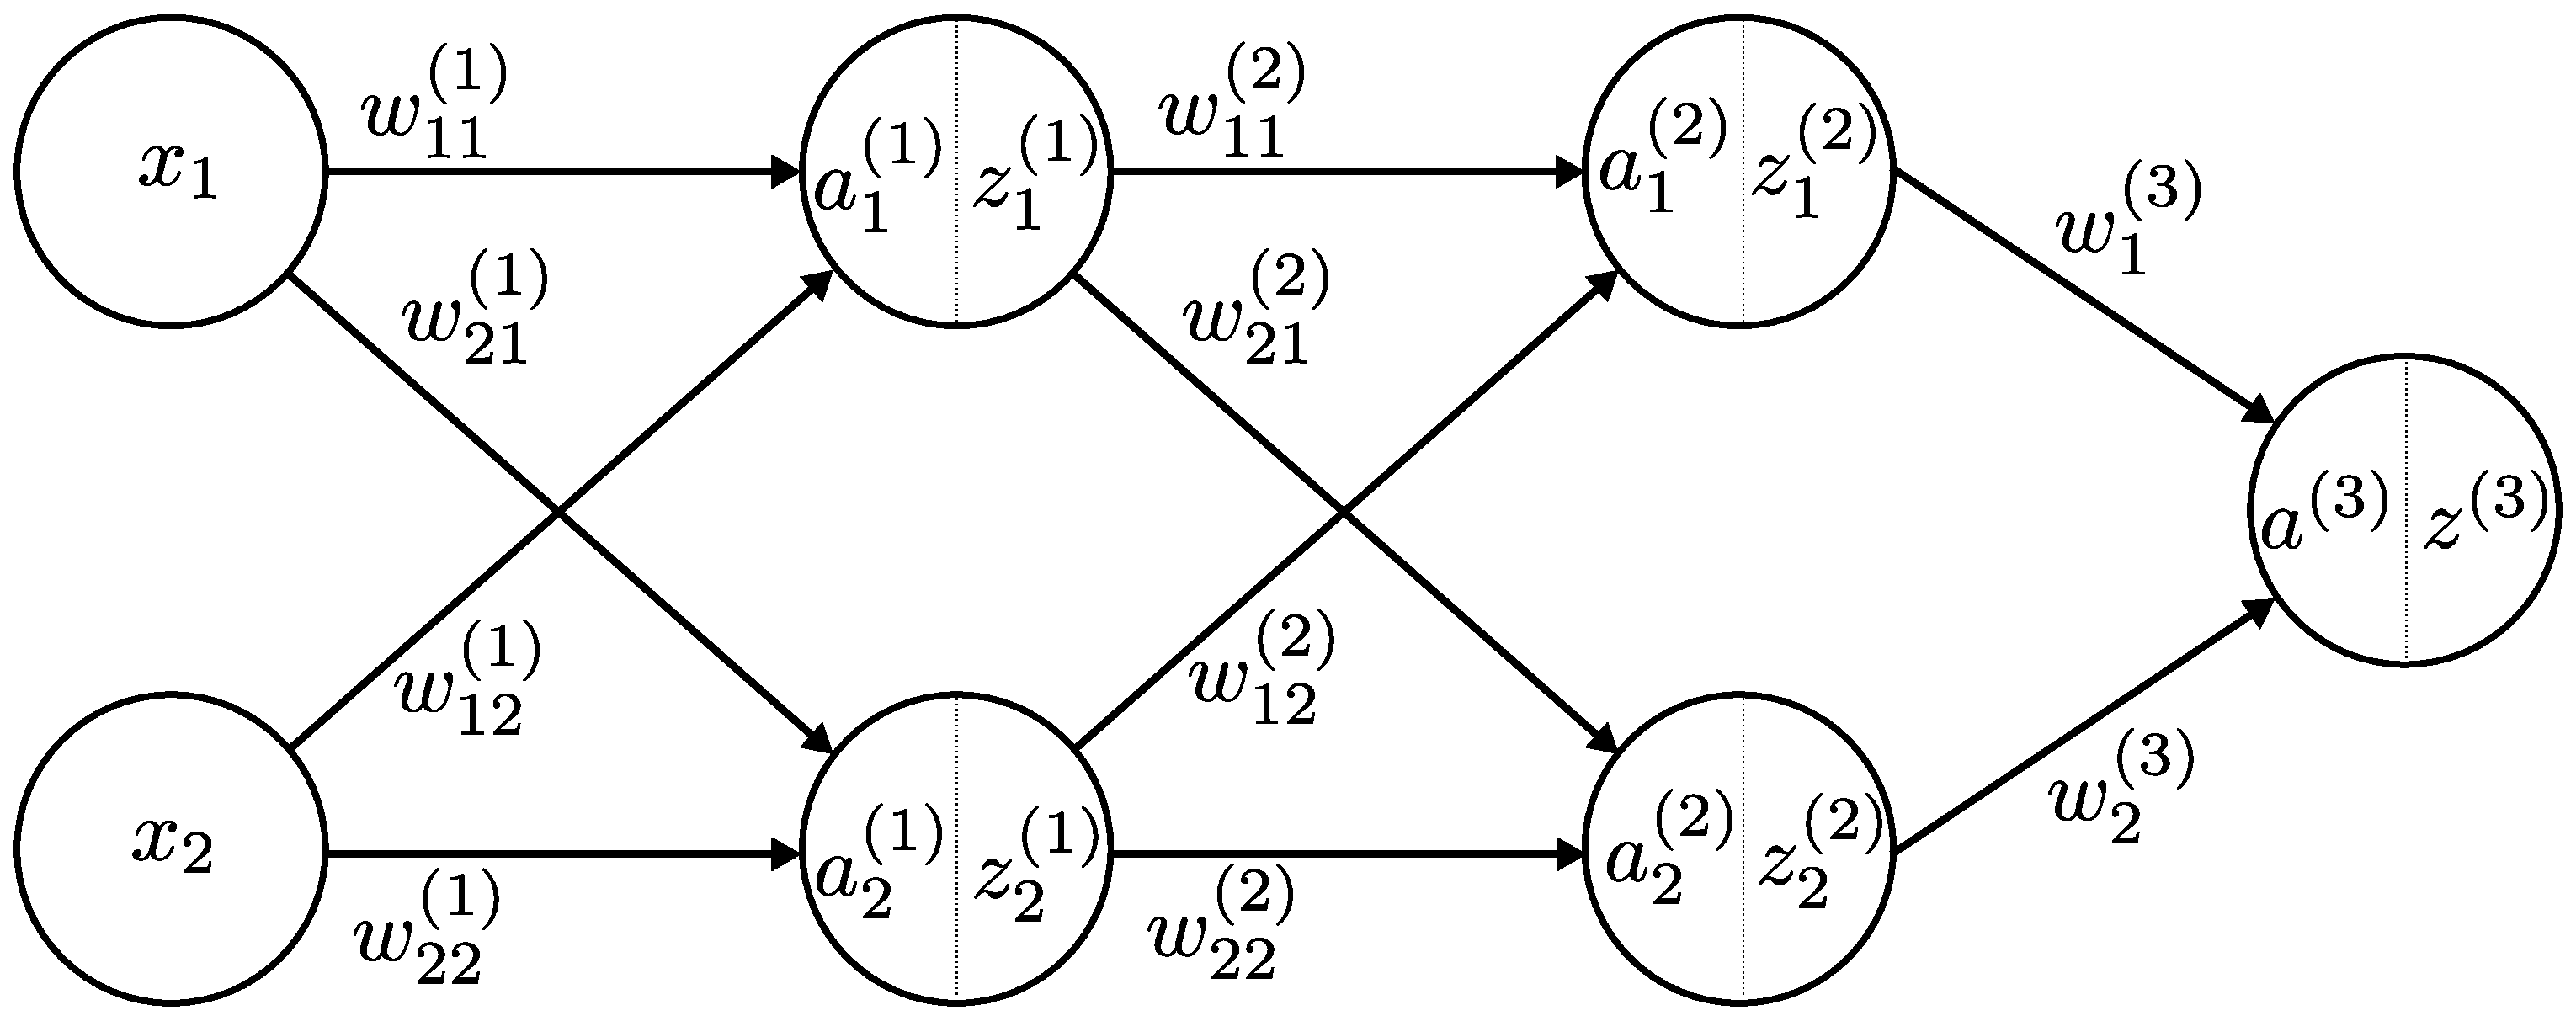
\includegraphics[width=0.9\textwidth]{./neural_networks.eps}
\caption{Example neural network}
\label{fig:nnexample}
\end{figure}

Let's start by defining what all of the pieces here mean. We have our inputs $x_i$, which we'll also refer to as the zero-th layer, so $z_i^{(0)} \triangleq x_i $. between the layers we have each set of weights, so $w_{ij}^{(k)}$ represents the weight from node $j$ in layer $k-1$ to node $i$ in layer $k$. Each hidden layer is comprised of two parts (which are separated by a dotted line in Figure \ref{fig:nnexample}), the activations $a_i^{(k)}$ and the hidden node values $z_i^{(k)}$. The activations are the sum of the incoming paths into the node: the value of the last layer times the weight along the path. For example, $a_1^{(1)}=x_1 w_{11}^{(1)} + x_2 w_{12}^{(2)}$. The hidden node values are then the activations transformed by an activation function. While there are many choices for this including sigmoids, hyperbolic tangent, and more recently rectified linear units (ReLU), we'll represent the general case of activations with $\sigma(\cdot)$. Using this, the hidden node value can be defined as:

\begin{equation}
    z_i^{(k)} = \sigma(a_i^{(k)})
\end{equation}

So for our example in in Figure \ref{fig:nnexample} wiht $a_1^{(1)}$, we could write out the expression to "feed forward" from one layer into the next in one line:

\begin{equation}
    z_1^{(k)} = \sigma(a_i^{(k)}) = \sigma(x_1 w_{11}^{(1)} + x_2 w_{12}^{(2)})
\end{equation}

\begin{figure}[h]
\centering
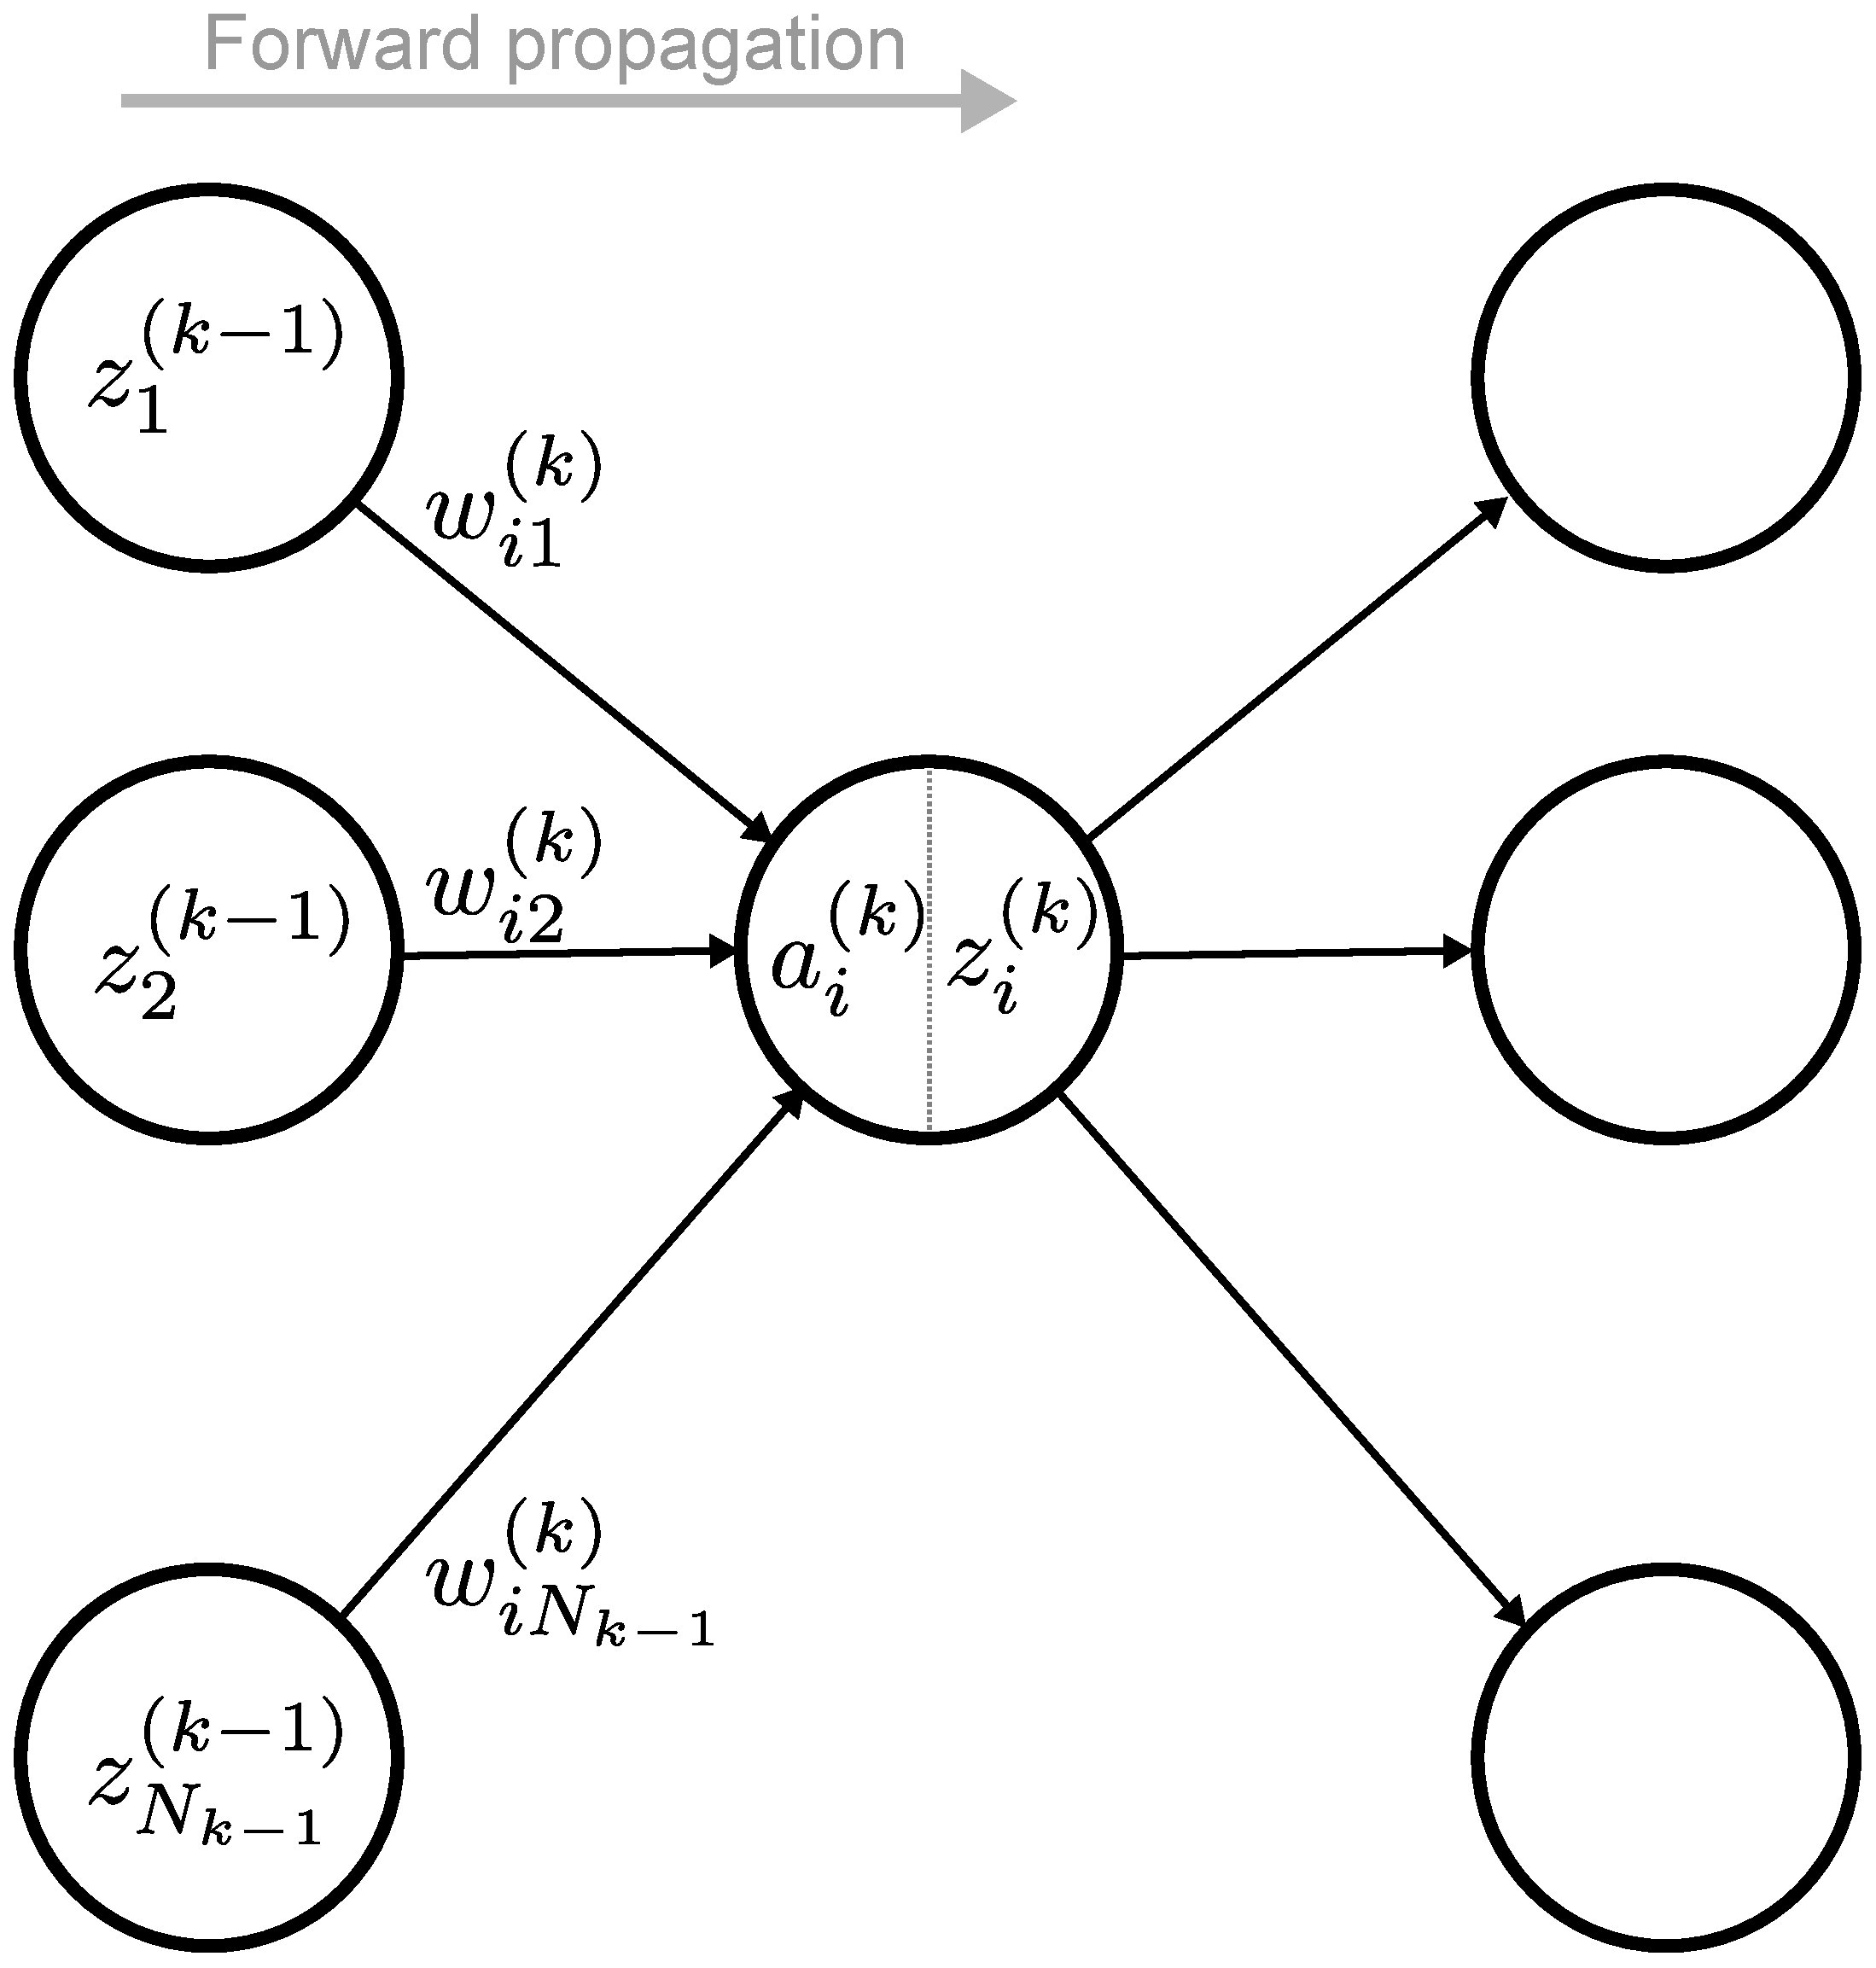
\includegraphics[width=0.45\textwidth]{./neural_networks_local_forward_propagation.eps}
\caption{Example neural network}
\label{fig:ff}
\end{figure}

We can do this for all of the nodes in the neural network feeding each layer forward into the next as demonstrated in Figure \ref{fig:ff}. More generally, we can write:

\begin{equation}
    a_i^{(k)} = \sum_{j=1}^{N_{k-1}} w_{ij}^{(k)} z_j^{(k-1)} 
\end{equation}

and

\begin{equation}
    z_i^{(k)} = \sigma(a_i^{(k)})
\end{equation}

Which collectively feed each layer forward to the next. This will fully populate the neural network values for a given set of weights. Let's adopt a matrix notation to store these and right them all out:

\begin{equation}
\mathbf{x} = 
    \begin{bmatrix}
        x_{1}\\
        x_{2}\\
        \vdots\\
        x_{N_{k}}\\
    \end{bmatrix}, \quad
    \mathbf{a}^{(k)} = 
    \begin{bmatrix}
        a_1^{(k)}\\
        a_2^{(k)}\\
        \vdots\\
        a_{N_k}^{(k)}\\
    \end{bmatrix}, \quad
    \mathbf{z}^{(k)} = 
    \begin{bmatrix}
        z_1^{(k)}\\
        z_2^{(k)}\\
        \vdots\\
        z_{N_k}^{(k)}\\
    \end{bmatrix}, \quad
    \mathbf{W}^{(k)} = 
    \begin{bmatrix}
        w_{11}^{(k)} & w_{12}^{(k)} & \cdots & w_{1 N_k}^{(k)}\\[2ex]
        w_{21}^{(k)} & w_{22}^{(k)} & \cdots & w_{2 N_k}^{(k)}\\[2ex]
        \vdots & \vdots &  & \vdots\\[2ex]
        w_{N_{k+1} 1}^{(k)} & w_{N_{k+1} 2}^{(k)} & \cdots & w_{N_{k+1} N_k }^{(k)}\\[2ex]
    \end{bmatrix}
\end{equation}

Each layer has its own collection of activations, hidden node values, and weights.

In this document all scalars are represented with normal text (e.g. $x$) vectors are represented in bold text (e.g. $\mathbf{x}$) and are assumed to be column vectors (e.g. $[N \times 1]$), matrices are represented as bold capital letters (e.g. $\mathbf{X}$). Subscripts index rows and columns of matrices and superscripts enclosed in parentheses differentiate between matrices (in this case, associated with different layers of the neural network). For example, $x_{ij}^{(k)}$ refers to element in row $i$ and column $j$ of matrix $\mathbf{X}^{(k)}$.

We start by calculating the error resulting from passing a value through the network.







\begin{equation}
\mathbf{x} = 
    \begin{bmatrix}
        x_{1}\\
        x_{2}\\
        \vdots\\
        x_{N_{k}}\\
    \end{bmatrix}
\end{equation}

$\mathbf{z}^{(0)} \triangleq \mathbf{x}$

\begin{equation}
\bm{\delta}^{(k)} = 
    \begin{bmatrix}
        \delta_1^{(k)}\\
        \delta_2^{(k)}\\
        \vdots\\
        \delta_{N_k}^{(k)}\\
    \end{bmatrix}
\end{equation}

\begin{equation}
\mathbf{z}^{(k)} = 
    \begin{bmatrix}
        z_1^{(k)}\\
        z_2^{(k)}\\
        \vdots\\
        z_{N_k}^{(k)}\\
    \end{bmatrix}
\end{equation}

\begin{equation}
\mathbf{W}^{(k)} = 
    \begin{bmatrix}
        w_{11}^{(k)} & w_{12}^{(k)} & \cdots & w_{1 N_k}^{(k)}\\[2ex]
        w_{21}^{(k)} & w_{22}^{(k)} & \cdots & w_{2 N_k}^{(k)}\\[2ex]
        \vdots & \vdots &  & \vdots\\[2ex]
        w_{N_{k+1} 1}^{(k)} & w_{N_{k+1} 2}^{(k)} & \cdots & w_{N_{k+1} N_k }^{(k)}\\[2ex]
    \end{bmatrix}
\end{equation}





\begin{figure}[h]
\centering
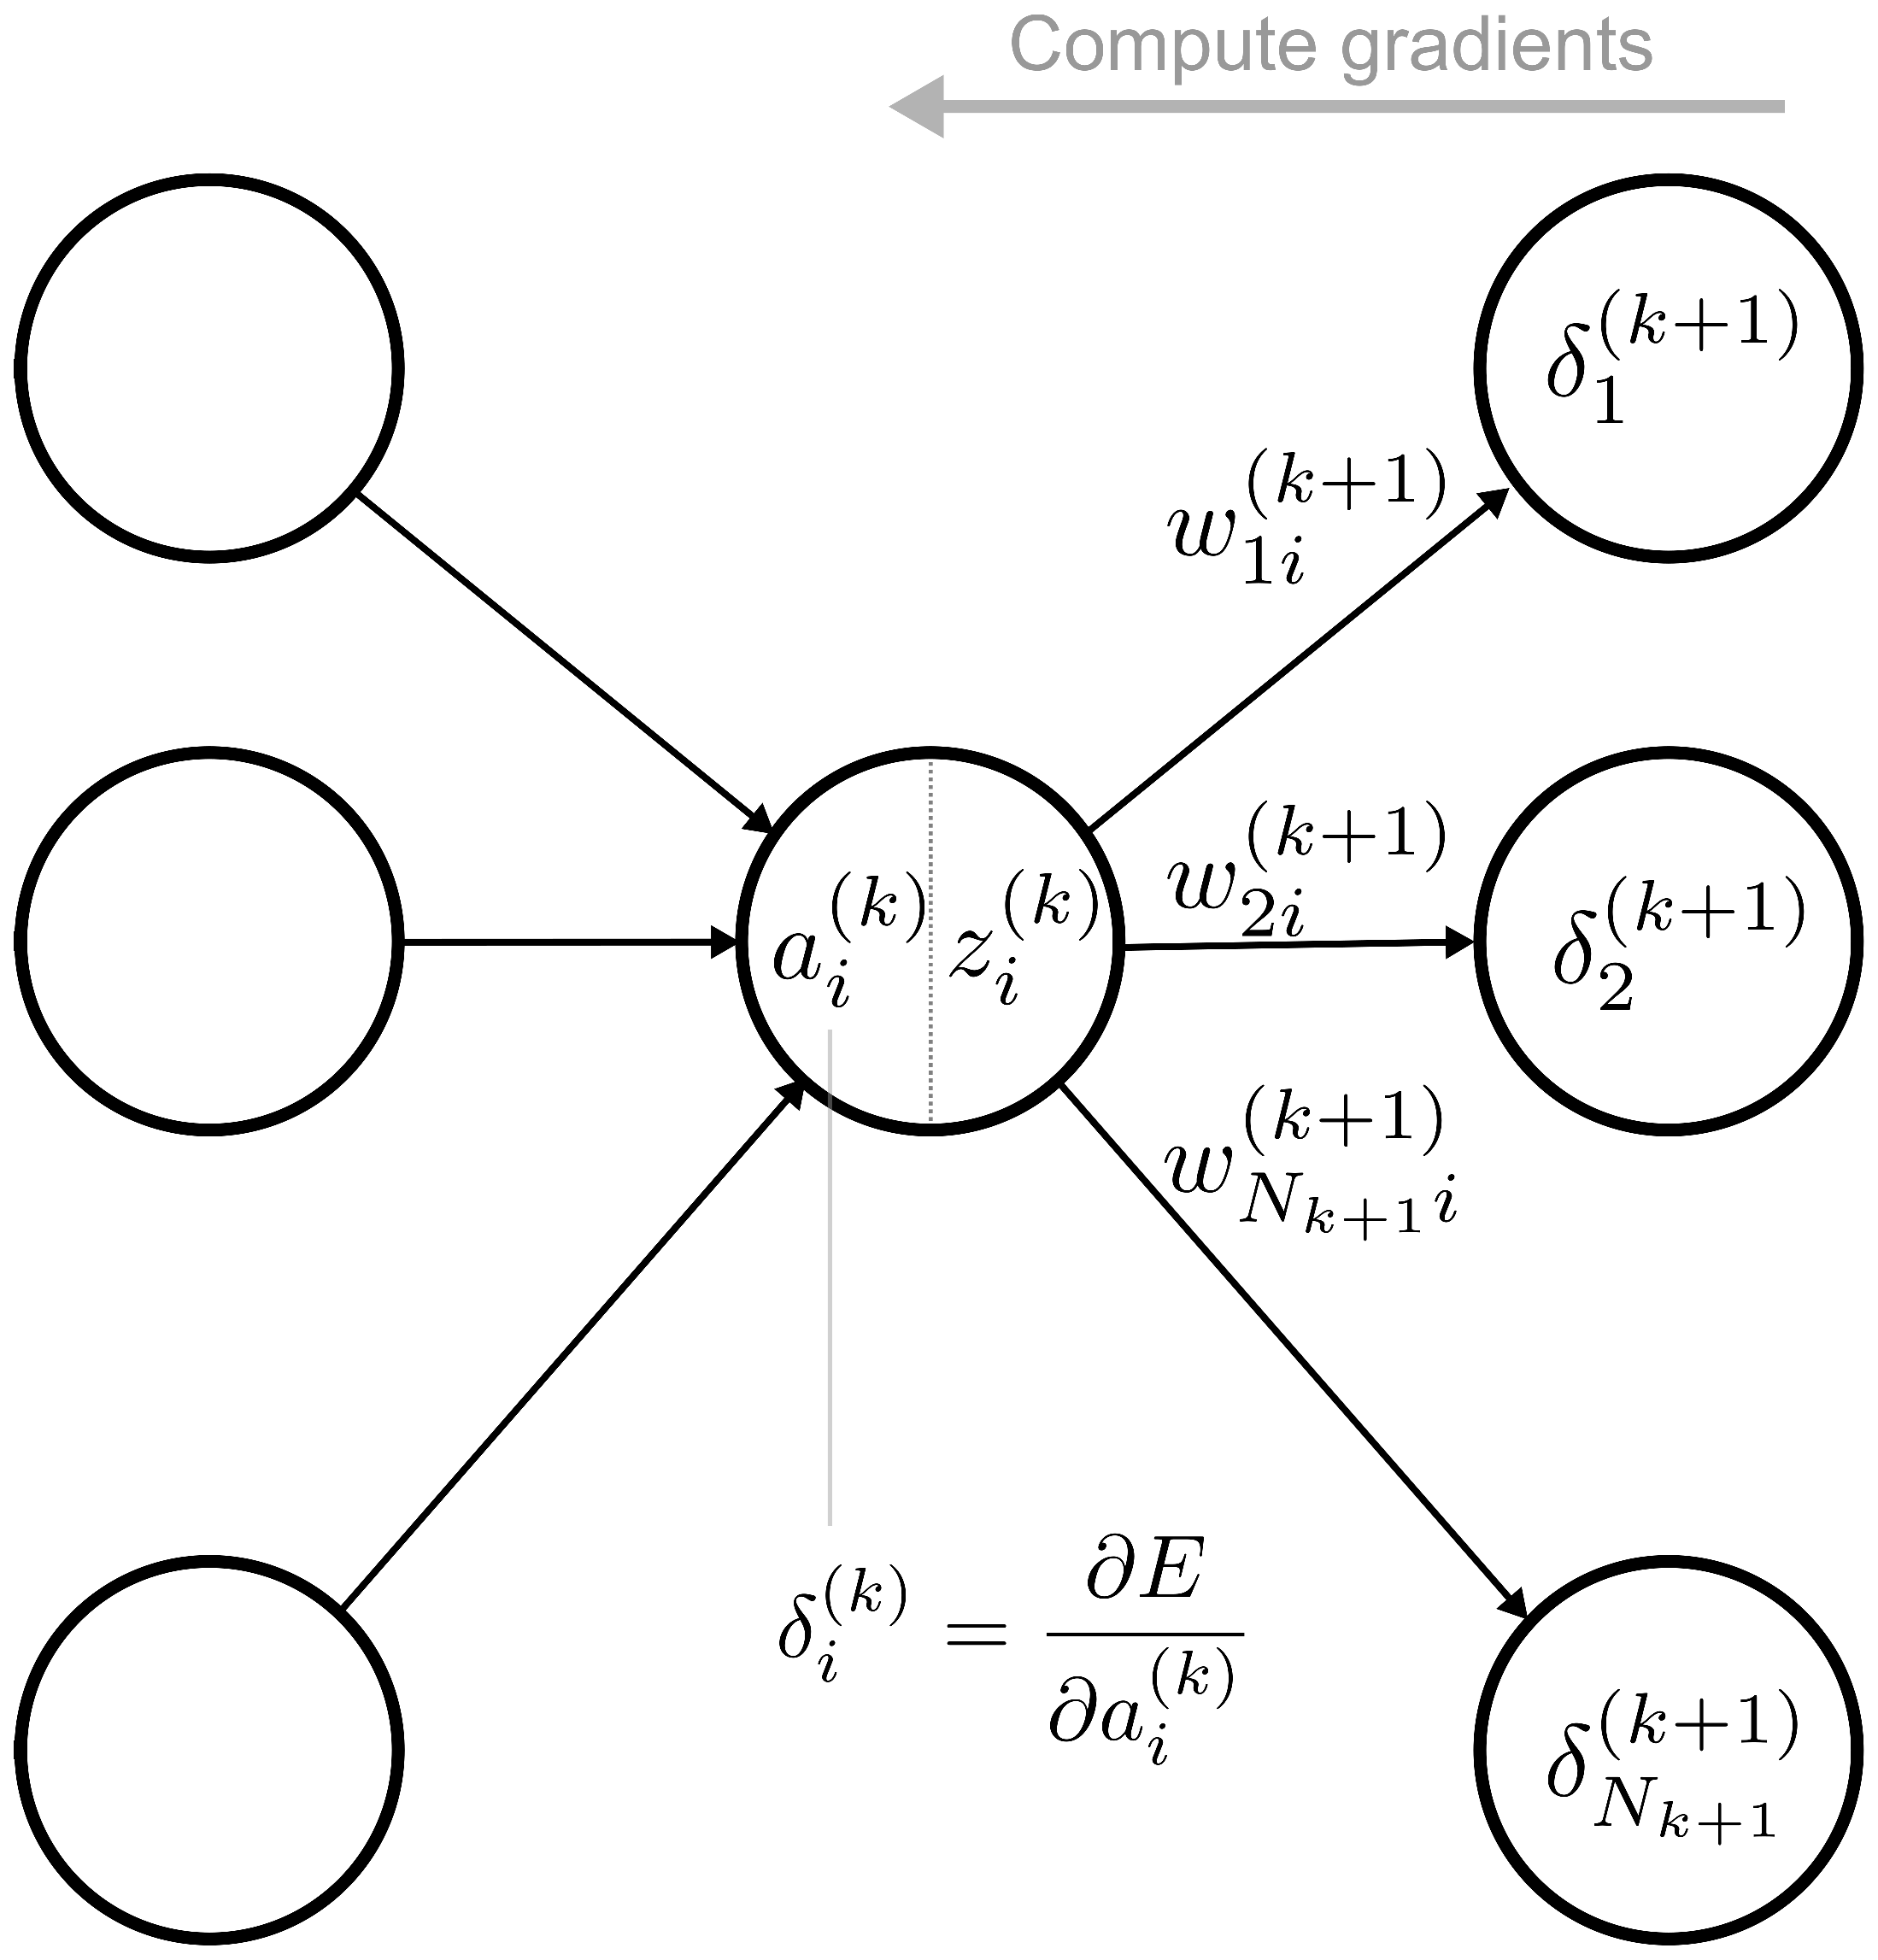
\includegraphics[width=0.45\textwidth]{./neural_networks_local_backpropagation.eps}
\caption{Example neural network}
\end{figure}

\begin{figure}[h]
\centering
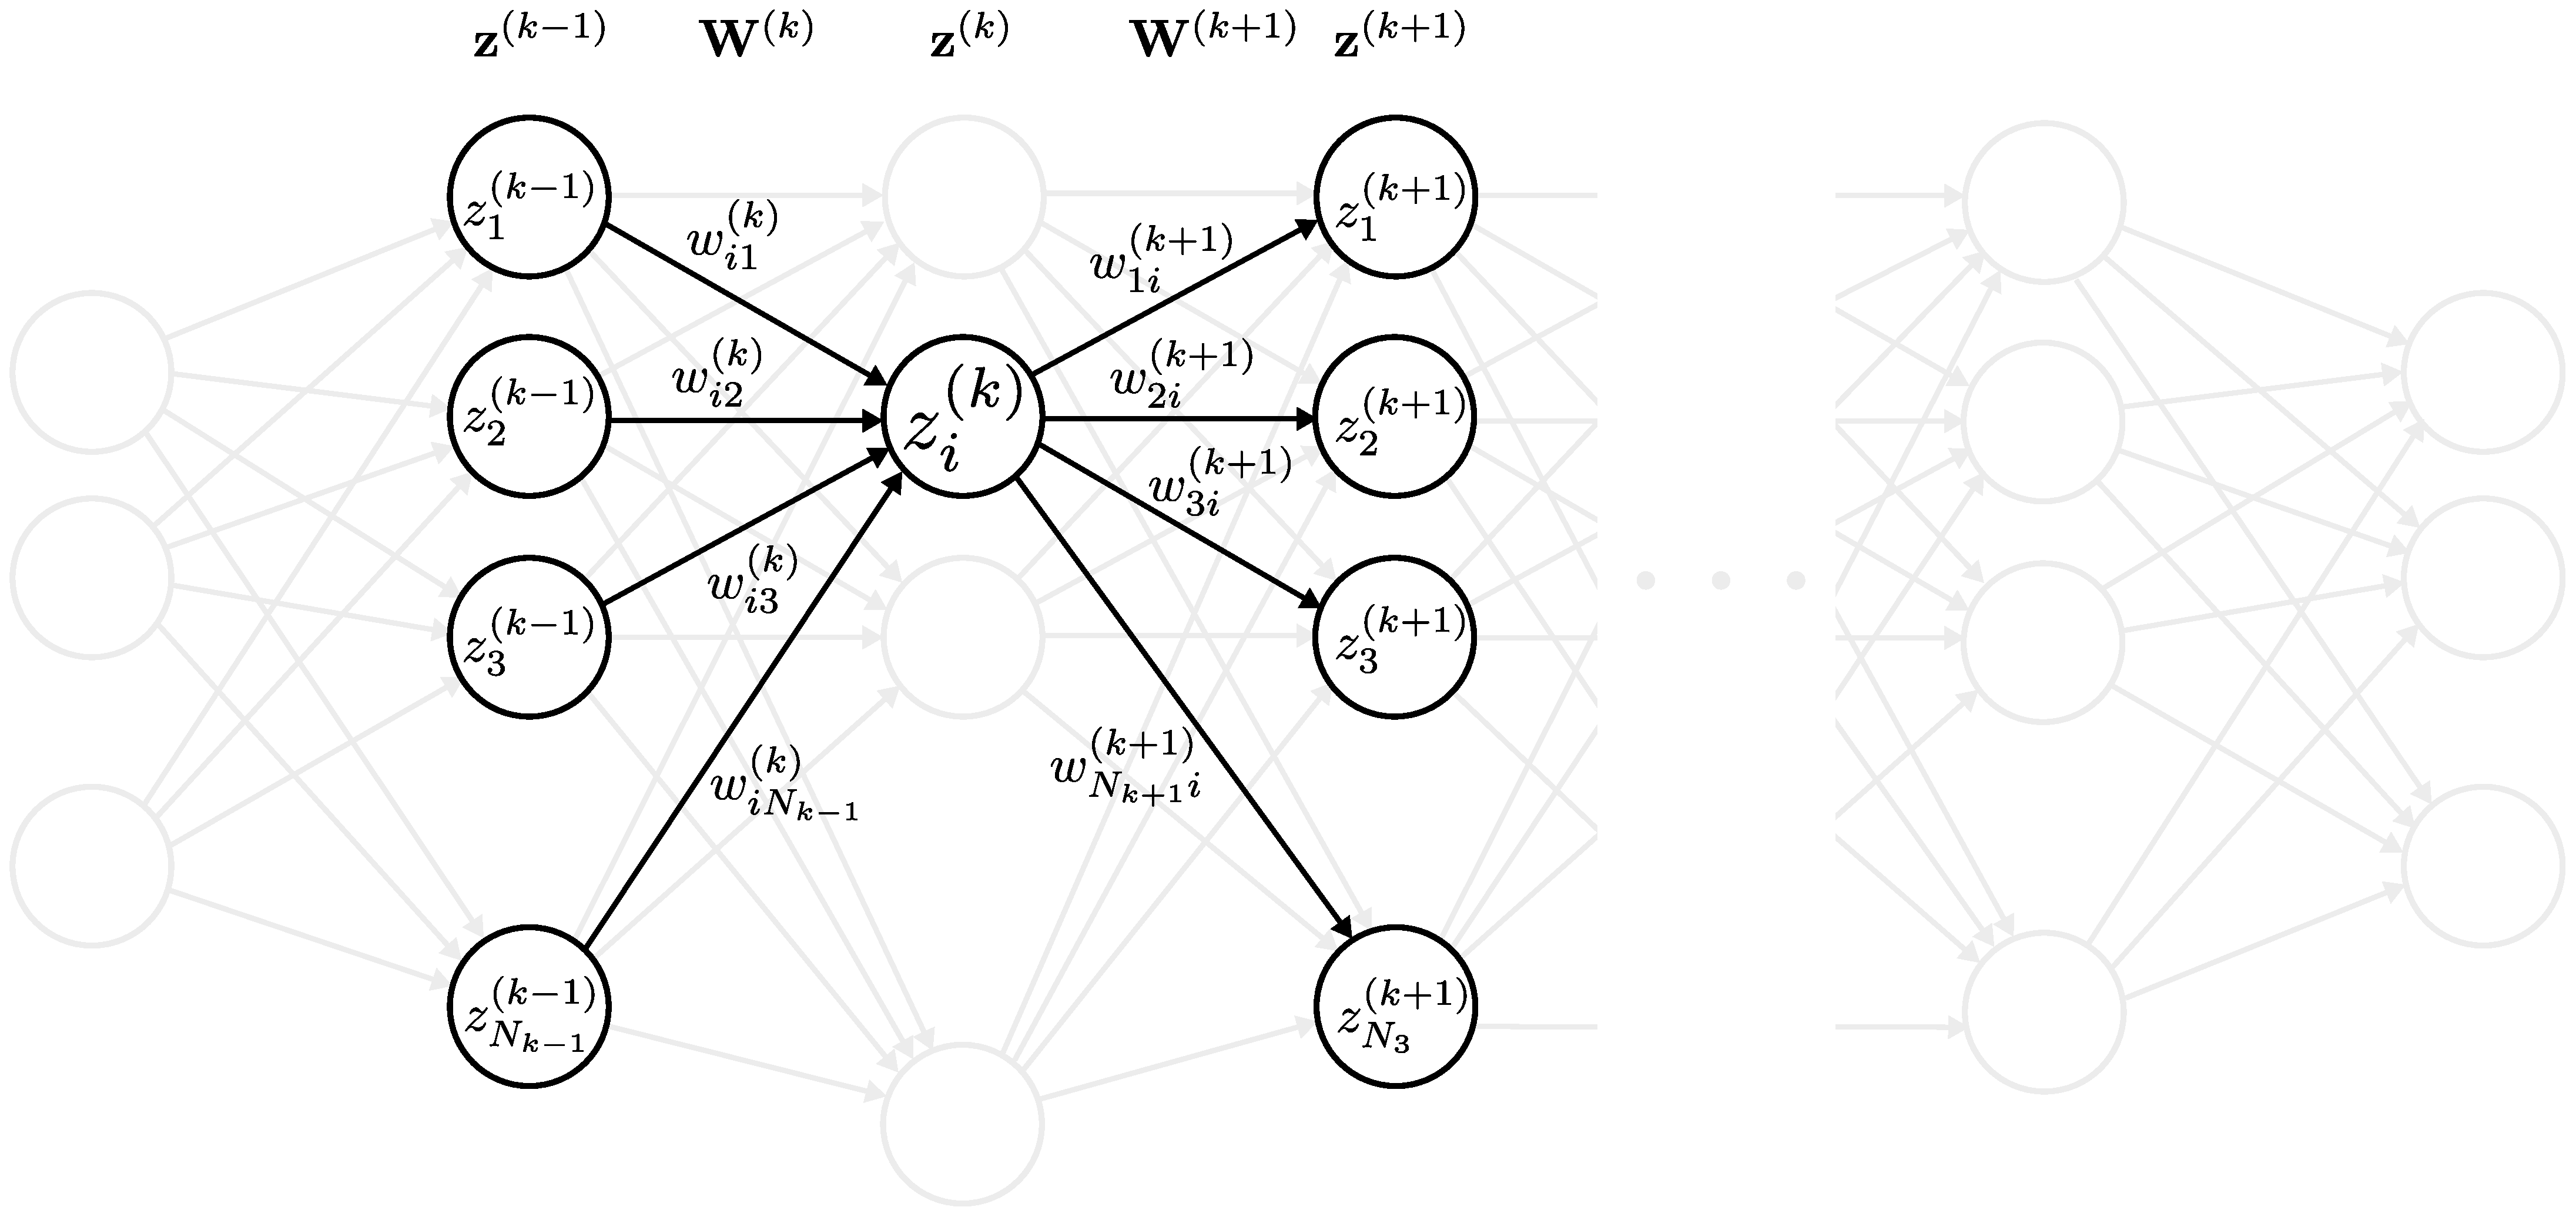
\includegraphics[width=0.9\textwidth]{./neural_networks_full_focused_example.eps}
\caption{Example neural network}
\end{figure}

\begin{figure}[h]
\centering
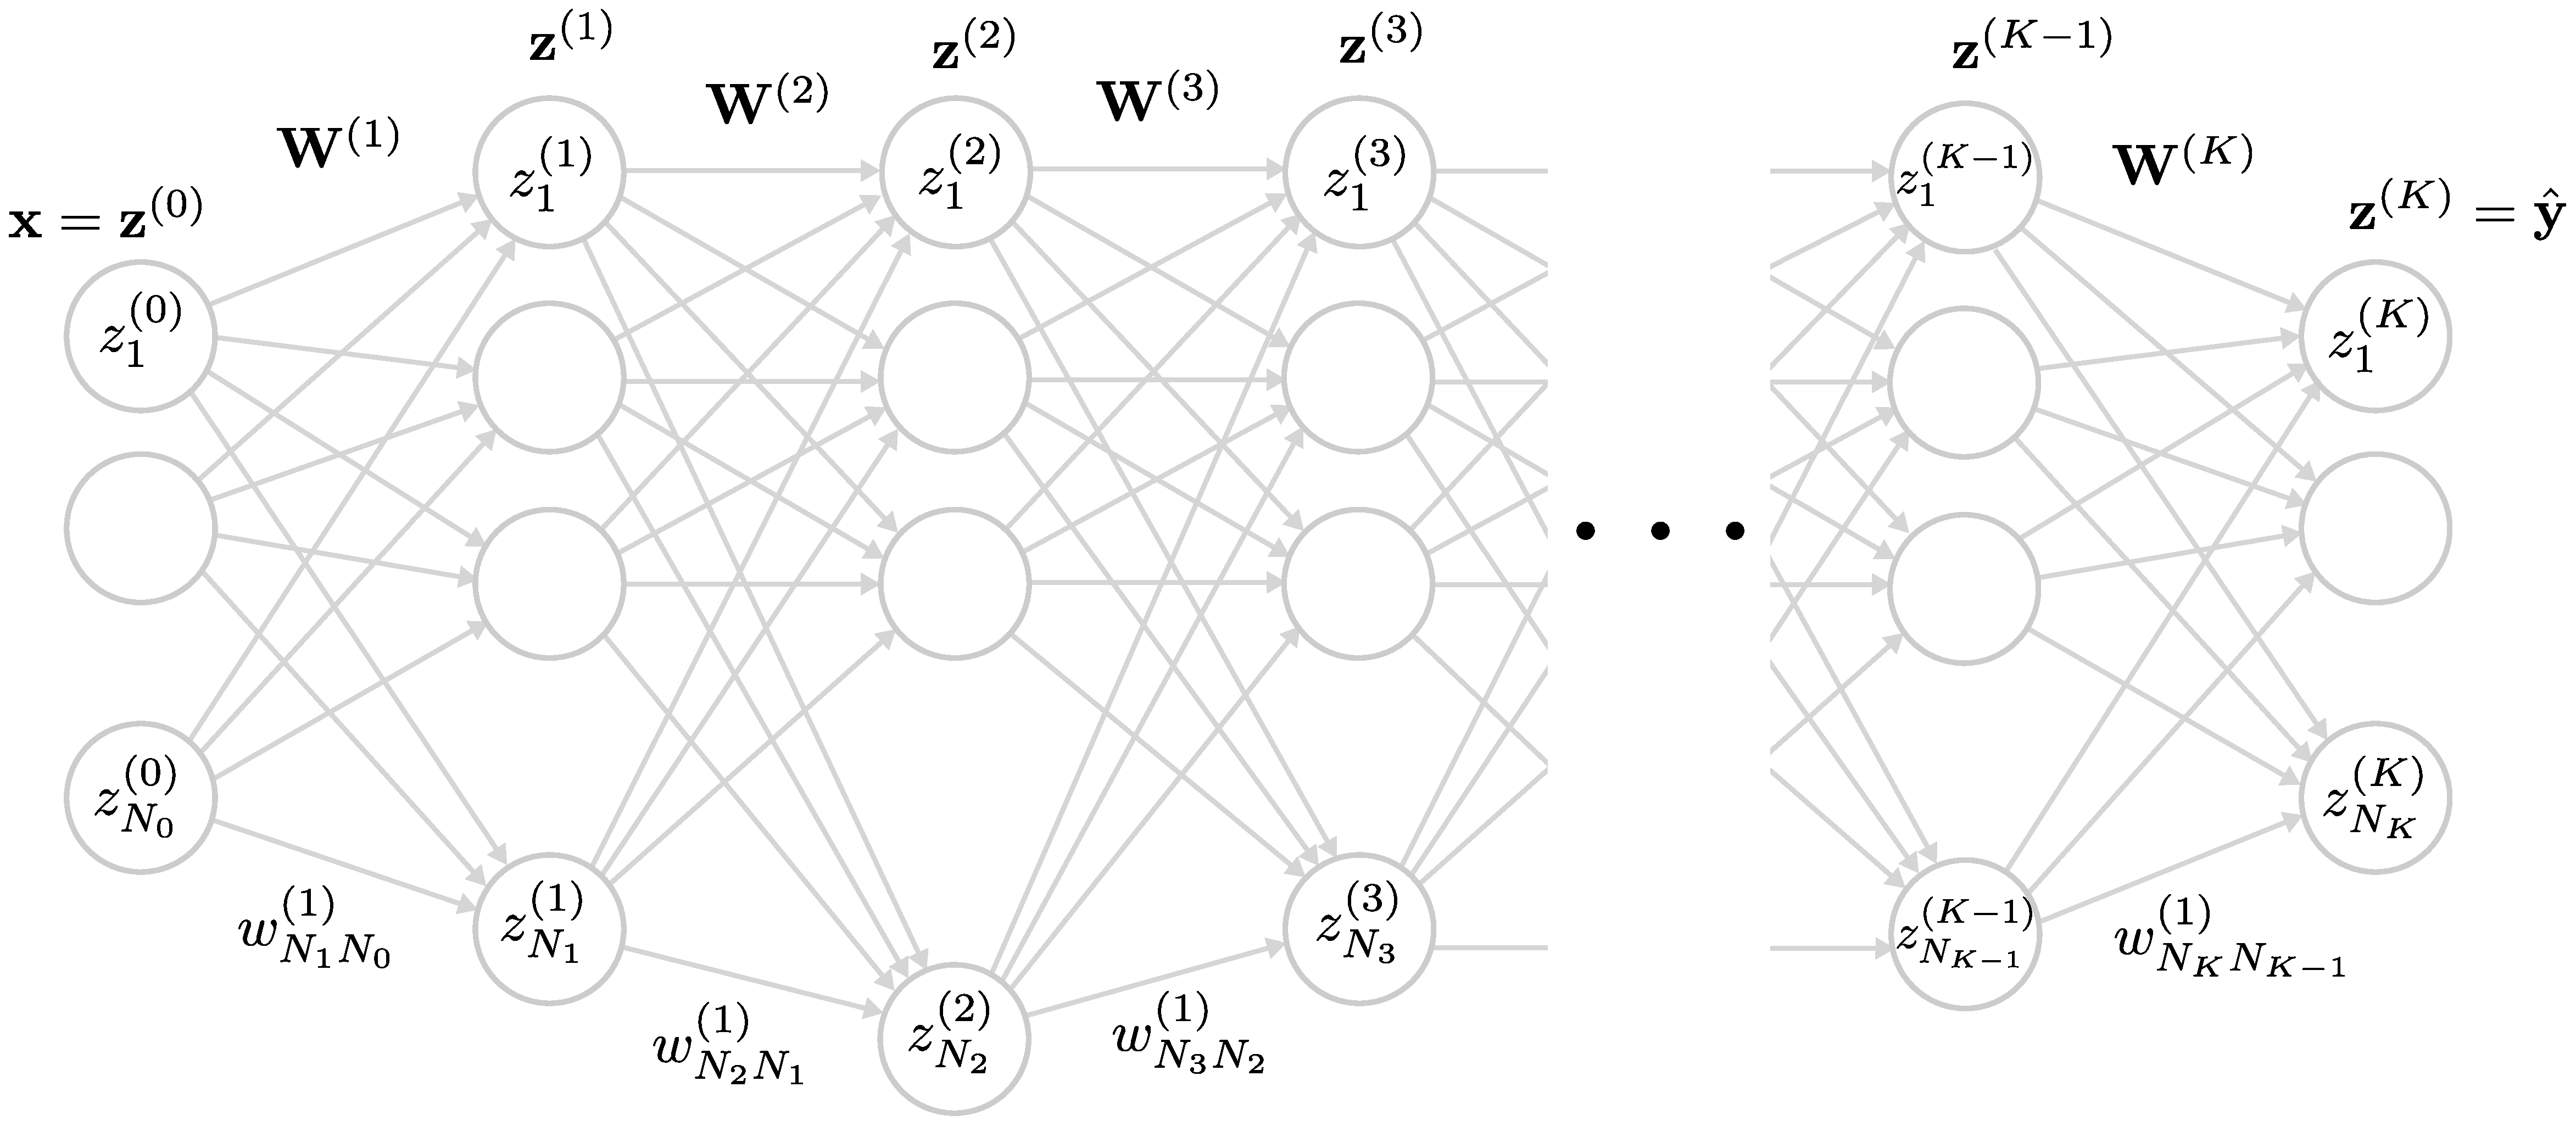
\includegraphics[width=0.9\textwidth]{./neural_networks_full_with_labels.eps}
\caption{Example neural network}
\end{figure}


\begin{table}[h]
\centering
\caption{Backpropagation Step-by-step}
\begin{tabular}{llllll}
\toprule
\emph{Step} & \emph{Var} & \emph{Local Relationship} & \emph{Local Derivative} & \emph{Backpropagated Derivative} & \\
\midrule
1 & $z^{(3)}$ & $E_n = \frac{1}{2}(z^{(3)} - y)^2$ & 
$\dfrac{\partial E_n}{\partial z^{(3)}} = z^{(3)} - y$ & 
$\dfrac{\partial E_n}{\partial z^{(3)}} = $ & 
$z^{(3)} - y$ \\[4ex]

2 & $a^{(3)}$ & 
$z^{(3)}=\sigma(a^{(3)})$ & 
$\dfrac{\partial z^{(3)}}{\partial a^{(3)}} = \sigma^{'}(a^{(3)})$ & 
$\dfrac{\partial E_n}{\partial a^{(3)}} = \dfrac{\partial E_n}{\partial z^{(3)}} \dfrac{\partial z^{(3)}}{\partial a^{(3)}}=$ & 
$(z^{(3)} - y) \sigma^{'}(a^{(3)}) \triangleq \delta^{(3)}$ \\[4ex]

3 & $z_i^{(2)}$ & $a^{(3)} = \sum\limits_{j=1}^{N_2} w_j^{(3)} z_j^{(2)}$ & $\dfrac{\partial a^{(3)}}{\partial z_i^{(2)}}= w_i^{(3)}$ & $\dfrac{\partial E_n}{\partial z_i^{(2)}} = \dfrac{\partial E_n}{\partial a^{(3)}} \dfrac{\partial a^{(3)}}{\partial z_i^{(2)}}=$ & 
$ \delta^{(3)} w_i^{(3)}$ \\[4ex]

4 & $a_i^{(2)}$ & 
$z_i^{(2)} = \sigma(a_i^{(2)})$ & 
$\dfrac{\partial z_i^{(2)}}{\partial a_i^{(2)}}= \sigma^{'}(a_i^{(2)})$ & 
$\dfrac{\partial E_n}{\partial a_i^{(2)}} = \dfrac{\partial E_n}{\partial z_i^{(2)}} \dfrac{\partial z_i^{(2)}}{\partial a_i^{(2)}} =$ & 
$\delta^{(3)} w_i^{(3)} \sigma^{'}(a_i^{(2)}) \triangleq \delta_i^{(2)}$ \\[4ex]

5 & $z_i^{(1)}$ &
$a_j^{(2)} = \sum\limits_{k=1}^{N_1} w_{jk}^{(2)} z_k^{(1)}$ & 
$\dfrac{\partial a_j^{(2)}}{\partial z_i^{(1)}} = w_{ji}^{(2)}$ & 
$\dfrac{\partial E_n}{\partial z_i^{(1)}} = \sum\limits_{j=1}^{N_2}\dfrac{\partial E_n}{\partial a_j^{(2)}} \dfrac{\partial a_j^{(2)}}{\partial z_i^{(1)}} =$ & 
$\sum\limits_{j=1}^{N_2} \delta_j^{(2)} w_{ji}^{(2)}$\\[4ex]

6 & $a_i^{(1)}$ & 
$z_i^{(1)} = \sigma(a_i^{(1)})$ &
$\dfrac{\partial z_i^{(1)}}{\partial a_i^{(1)}} = \sigma^{'}(a_i^{(1)})$ &
$\dfrac{\partial E_n}{\partial a_i^{(1)}} = \dfrac{\partial E_n}{\partial z_i^{(1)}} \dfrac{\partial z_i^{(1)}}{\partial a_i^{(1)}}= $& 
$\sigma^{'}(a_i^{(1)}) \sum\limits_{j=1}^{N_2} \delta_j^{(2)} w_{ji}^{(2)} \triangleq \delta_i^{(1)}$ \\[4ex]

7 & $x_i$ &
$a_j^{(1)} = \sum\limits_{k=1}^{N_0} w_{jk}^{(1)} x_k$ & 
$\dfrac{\partial a_j^{(1)}}{\partial z_i^{(0)}} = w_{ji}^{(1)}$ & 
$\dfrac{\partial E_n}{\partial x_i} = \sum\limits_{j=1}^{N_1}\dfrac{\partial E_n}{\partial a_j^{(1)}} \dfrac{\partial a_j^{(1)}}{\partial x_i} =$ & 
$\sum\limits_{j=1}^{N_1} \delta_j^{(1)} w_{ji}^{(1)}$ \\[4ex]

\bottomrule
\end{tabular}
\end{table}





% This table is for the matrix forms of the backpropagation equations
\begin{table}[h]
\centering
\caption{Backpropagation Step-by-step}
\begin{tabular}{lll}
\toprule
\emph{ID} & \emph{Derivative} & \emph{Matrix Forms} \\
\midrule
1 & $\dfrac{\partial E_n}{\partial z^{(3)}} =$ & $z^{(3)} - y$ \\[4ex]

2 & $\dfrac{\partial E_n}{\partial a^{(3)}} = \dfrac{\partial E_n}{\partial z^{(3)}} \dfrac{\partial z^{(3)}}{\partial a^{(3)}}=$ & $(z^{(3)} - y) \sigma^{'}(a^{(3)}) \triangleq \delta^{(3)}$  \\[4ex]

3 & $\dfrac{\partial E_n}{\partial \mathbf{z}^{(2)}} = \dfrac{\partial E_n}{\partial a^{(3)}} \dfrac{\partial a^{(3)}}{\partial \mathbf{z}^{(2)}} =$ & $ \delta^{(3)} \mathbf{w}^{(3)}$  \\[4ex]

4 & $\dfrac{\partial E_n}{\partial \mathbf{a}^{(2)}} = \dfrac{\partial E_n}{\partial \mathbf{z}^{(2)}} \dfrac{\partial \mathbf{z}^{(2)}}{\partial \mathbf{a}^{(2)}} =$ & $ \delta^{(3)} \mathbf{w}^{(3)} \circ \sigma^{'}(\mathbf{a}^{(2)}) \triangleq \bm{\delta}^{(2)}$  \\[4ex]

5 & $\dfrac{\partial E_n}{\partial \mathbf{z}^{(1)}} = \dfrac{\partial E_n}{\partial \mathbf{a}^{(2)}} \dfrac{\partial \mathbf{a}^{(2)}}{\partial \mathbf{z}^{(1)}}=$ & $ {\mathbf{W}^{(2)}}^{\top} \bm{\delta}^{(2)}$  \\[4ex]

6 &  $\dfrac{\partial E_n}{\partial \mathbf{a}^{(1)}} = \dfrac{\partial E_n}{\partial \mathbf{z}^{(1)}} \dfrac{\partial \mathbf{z}^{(1)}}{\partial \mathbf{a}^{(1)}} =$ & $ {\mathbf{W}^{(2)}}^{\top} \bm{\delta}^{(2)} \circ \sigma^{'}(\mathbf{a}^{(1)}) \triangleq \bm{\delta}^{(1)}$ \\[4ex]

7 & $\dfrac{\partial E_n}{\partial \mathbf{x}} =\dfrac{\partial E_n}{\partial \mathbf{a}^{(1)}} \dfrac{\partial \mathbf{a}^{(1)}}{\partial \mathbf{x}}=$ & $ {\mathbf{W}^{(1)}}^{\top} \bm{\delta}^{(1)}$ \\[4ex]

\bottomrule
\end{tabular}
\end{table}


\begin{equation}
    a_i^{(k)} = \sum_{j=1}^{N_{k-1}} w_{ij}^{(k)} z_j^{(k-1)} 
\end{equation}

\begin{equation}
    \mathbf{a}^{(k)} = \mathbf{W}^{(k)} \mathbf{z}^{(k-1)}
\end{equation}

\begin{equation}
    z_i^{(k)} = \sigma(a_i^{(k)})
\end{equation}

\begin{equation}
    \mathbf{z}^{(k)} = \sigma(\mathbf{a}^{(k)})
\end{equation}

\begin{equation}
    \dfrac{\partial a_i^{(k)}}{\partial w_{ij}^{(k-1)}} = z_j^{(k-1)}
\end{equation}


\begin{equation}
    \dfrac{\partial E_n}{\partial w_{ij}^{(k)}} = 
    \dfrac{\partial E_n}{\partial a_i^{(k)}} \dfrac{\partial a_i^{(k)}}{\partial w_{ij}^{(k)}} = \delta_i^{(k)} z_j^{(k-1)}
\end{equation}

\begin{equation}
    \dfrac{\partial E_n}{\partial \mathbf{w}^{(k)}} = \bm{\delta}^{(k)} {\mathbf{z}^{(k-1)}}^{\top}
\end{equation}

Where the $(i,j)^{\mathrm{th}}$ element of this matrix is $\frac{\partial E_n}{\partial w_{ij}}$.

\begin{equation}
\begin{split}
    \dfrac{\partial E_n}{\partial w_{ij}^{(k)}} &= 
    \dfrac{\partial E_n}{\partial a_i^{(k)}} \dfrac{\partial a_i^{(k)}}{\partial w_{ij}^{(k)}} \\
    &= \delta_i^{(k)} z_j^{(k-1)}
\end{split}
\end{equation}

\section{Definitions}




\end{document}


